\chapter{Results}\label{ch:results}

\par Here is where I will talk about what I have accomplished.\textbf{\textit{[This totally needs to be actually done]}}
\section{Simulation results, MATLAB}
\par MATLAB was initially used in developing the modified CEs, both with the RLM training method and the NSE training method. As such, the SNR profile that was used in testing was a simple slow-fading channel. A plot of the SNR profile is shown in Figure \ref{fig:matlabSNRProf}. 

\begin{figure}[ht]
\centering
\includegraphics[scale=1]{figures/matlab_sim_results/snrPRofile_matlabsim.eps}
\caption{SNR profile used in MATLAB simulation.}
\label{fig:matlabSNRProf}
\end{figure}

\par While there are six different fitness score weightings (as shown in Table \ref{table:fitMissions}), the flight tests conducted in \cite{tim_implementation} focused on Emergency, Cooperation and Power Saving. Because of this, these were the missions that the simulation focused on as well. Figure \ref{res:matSimFitscore} shows how the fitness score evolved over time during the simulation.

\begin{figure}[ht]
\begin{center}
\begin{subfigure}{\linewidth}
\centering
\includegraphics[scale=1]{figures/matlab_sim_results/fitObserved_emer.eps}
\end{subfigure}
\end{center}
\begin{center}
\begin{subfigure}{\linewidth}		
\centering
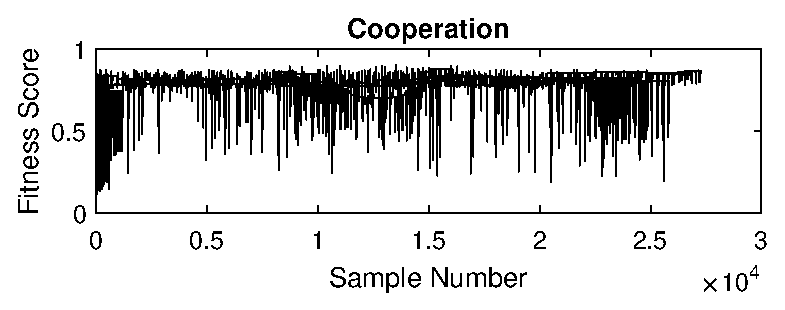
\includegraphics[scale=1]{figures/matlab_sim_results/fitObserved_coop.eps}
\end{subfigure}
\end{center}
\begin{center}
\begin{subfigure}{\linewidth}
	\centering
	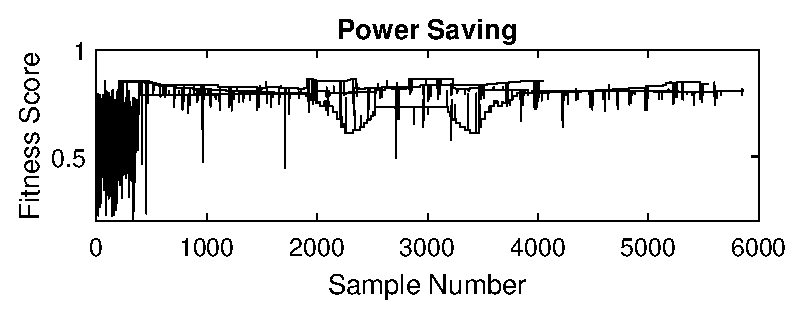
\includegraphics[scale=1]{figures/matlab_sim_results/fitObserved_powerSave.eps}
\end{subfigure}
\end{center}
\caption{Fitness score plotted over length of simulation.}\label{res:matSimFitscore}
\end{figure}
\par A few things are evident with the time series plots shown in \ref{res:matSimFitscore}. The first is that the spurs that are periodically showing up are the CE exploring random actions, and are spaced in a manner independent of training type. In addition, it is apparent that some mission types have different ranges of the action space, as the cooperation simulation has explorations that have a wider range of values than either the emergency simulation or the power saving simulation. Beyond this, it is evident that LM has a more difficult time than the other two training algorithms in adapting to the higher SNR portions of the simulated pass in both the cooperation and powersaving mission cases. Beyond this, it's fairly difficult to draw conclusions from the time series plots.
\begin{figure}
\centering
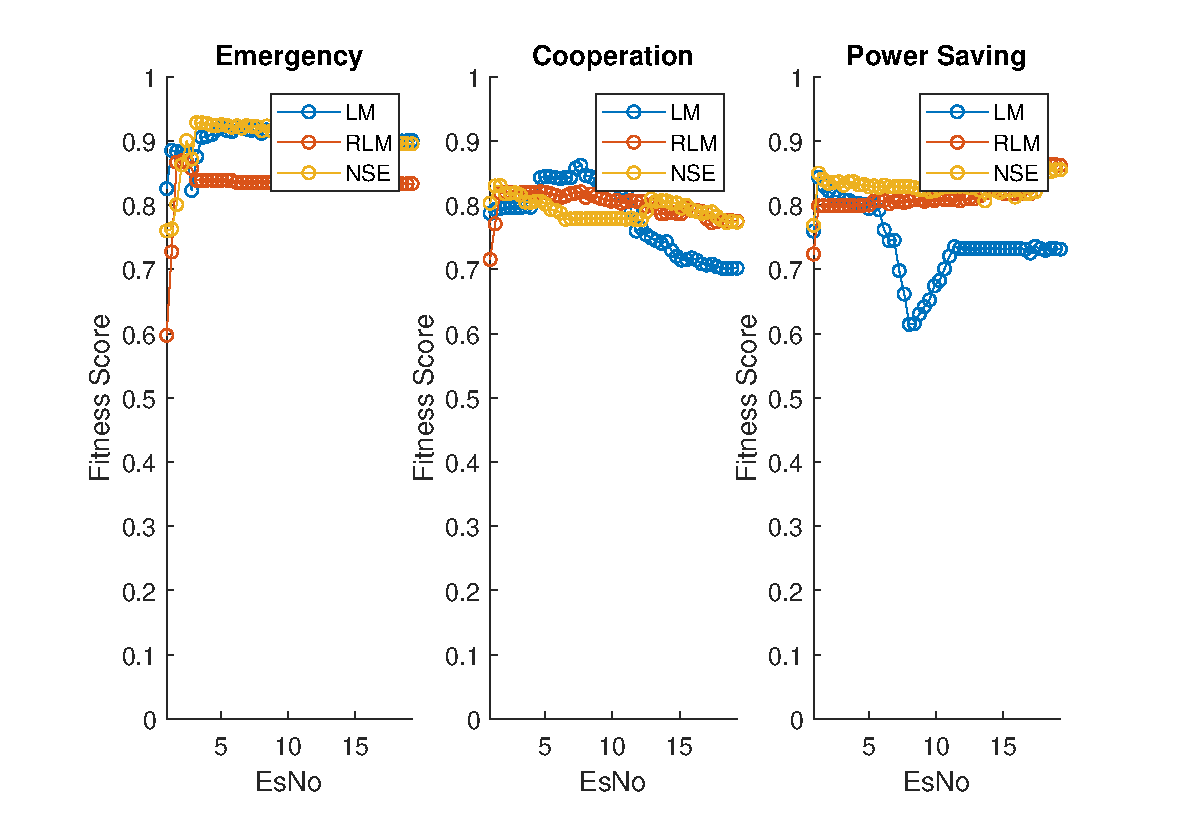
\includegraphics[width=\textwidth]{figures/matlab_sim_results/binnedMeans_sim.eps}
\caption{Value taking the mean fitness value}
\label{res:matSimBinMean}
\end{figure}
\par In order to get a better understanding of the behavior of the different CEs, fitness scores were split into bins based on the EsNo at the moment that the fitness was observed. Once this was done, the mean was taken within each bin. This plot is shown in Figure \ref{res:matSimBinMean}. For the Emergency mission, LM and NSE proved to have similar average fitness scores, with RLM having lower average fitness scores. the cooperation mission was more ambiguous, with RLM and NSE performing better than LM in the higher EsNo regime, and performing worse than LM in the middle EsNo regime. Finally, the power saving mission shows both LM and RLM working markedly better than LM in the entire regime.
\par With the results shown in this section, there was enough motivation to progress from the MATLAB simulation to simulation, ground testing, and flight testing in C++. 
% \newpage
\clearpage
\section{Simulation results, C++}
\section{Ground Test and Integration}
\begin{itemize}
	\item \textbf{\textit{[DISCUSS PRETRAINING]}}
	\item Time series plot.
	\item histogram
	\item rel histogram
	\item 2d hist, rel, log
	\item binned mean
	\item binned median
	\item sum of binned means and binned medians.
	\item Entire work in appendix.
\end{itemize}

\section{Flight Test results}

\begin{itemize}
	\item \textbf{\textit{[DISCUSS PRETRAINING]}}
	\item Time series plot.
	\item histogram
	\item rel histogram
	\item 2d hist, rel, log
	\item binned mean
	\item binned median
	\item sum of binned means and binned medians.
	\item Entire work in appendix.
\end{itemize}